\section{Numbering\-Policy Class Reference}
\label{classNumberingPolicy}\index{NumberingPolicy@{NumberingPolicy}}
Inheritance diagram for Numbering\-Policy::\begin{figure}[H]
\begin{center}
\leavevmode
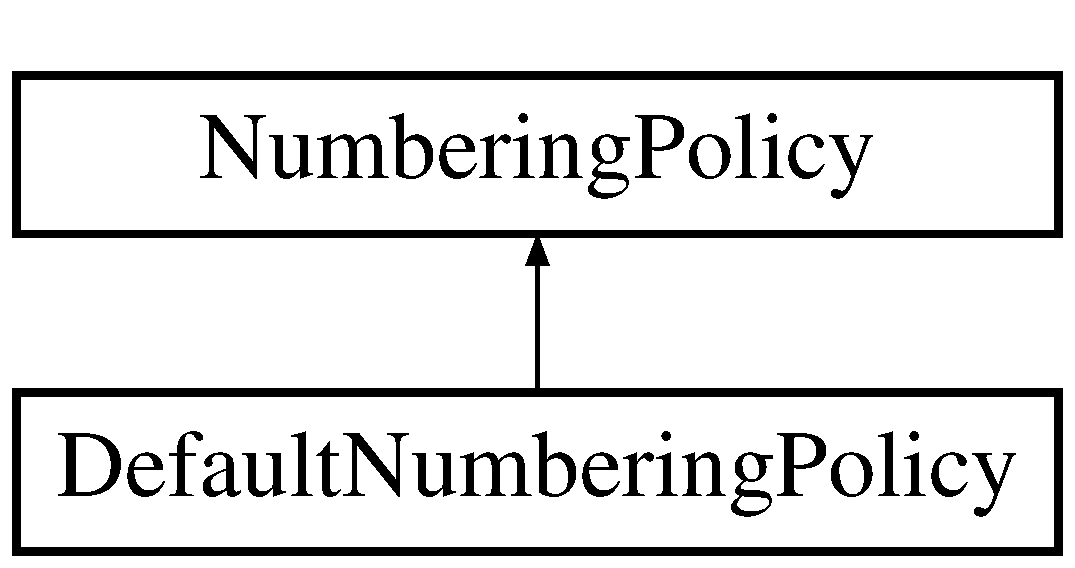
\includegraphics[height=2cm]{classNumberingPolicy}
\end{center}
\end{figure}
\subsection*{Public Member Functions}
\begin{CompactItemize}
\item 
{\bf \_\-\_\-del\_\-\_\-} ()
\item 
{\bf on\-Create} (obj)
\item 
{\bf on\-Delete} (obj)
\end{CompactItemize}


\subsection{Member Function Documentation}
\index{NumberingPolicy@{Numbering\-Policy}!__del__@{\_\-\_\-del\_\-\_\-}}
\index{__del__@{\_\-\_\-del\_\-\_\-}!NumberingPolicy@{Numbering\-Policy}}
\subsubsection{\setlength{\rightskip}{0pt plus 5cm}Numbering\-Policy::\_\-\_\-del\_\-\_\- ()}\label{classNumberingPolicy_NumberingPolicya0}




Reimplemented in {\bf Default\-Numbering\-Policy} {\rm (p.\,\pageref{classDefaultNumberingPolicy_DefaultNumberingPolicya0})}.\index{NumberingPolicy@{Numbering\-Policy}!onCreate@{onCreate}}
\index{onCreate@{onCreate}!NumberingPolicy@{Numbering\-Policy}}
\subsubsection{\setlength{\rightskip}{0pt plus 5cm}Numbering\-Policy::on\-Create (obj)}\label{classNumberingPolicy_NumberingPolicya1}




Reimplemented in {\bf Default\-Numbering\-Policy} {\rm (p.\,\pageref{classDefaultNumberingPolicy_DefaultNumberingPolicya1})}.\index{NumberingPolicy@{Numbering\-Policy}!onDelete@{onDelete}}
\index{onDelete@{onDelete}!NumberingPolicy@{Numbering\-Policy}}
\subsubsection{\setlength{\rightskip}{0pt plus 5cm}Numbering\-Policy::on\-Delete (obj)}\label{classNumberingPolicy_NumberingPolicya2}




Reimplemented in {\bf Default\-Numbering\-Policy} {\rm (p.\,\pageref{classDefaultNumberingPolicy_DefaultNumberingPolicya2})}.

The documentation for this class was generated from the following file:\begin{CompactItemize}
\item 
{\bf Numbering\-Policy.py}\end{CompactItemize}
